% ---------------------------
% Put these in your document preamble:
% ---------------------------
% \usepackage{graphicx}   % for \includegraphics
% \usepackage{float}      % for [H]
% \usepackage{placeins}   % for \FloatBarrier (keep floats from moving past a barrier)
% \usepackage{caption}    % if you need \captionof or extra caption control
% ---------------------------

% Appendix (body)
\chapter{Appendix} % Main appendix title
\label{Appendix}


% ======================================================================
% ======================================================================
% 
%
%                                Development
%
%
% ======================================================================
% % ======================================================================

% \section{Development Structure}
% \label{appendix:dev-structure}
% TODO --> Insert coding development structure here on how to utilize the package 
% correctly (maybe a README)


% ======================================================================
% ======================================================================
% 
%
%                                Tables
%
%
% ======================================================================
% % ======================================================================
\section{Fertility}
\label{annex:fertility-table}
Referenced on [\ref{sec:gen_efficiency}]\\

\begin{tabular}{rllr}
    \toprule
    New Tokens & Model & Type & Fertility \\
    \midrule
    0 & HuggingFaceTB/SmolLM2-135M & Baseline & 2.47 \\
    1000 & HuggingFaceTB/SmolLM2-135M & No Training & 1.94 \\
    1000 & HuggingFaceTB/SmolLM2-135M & With Training & 1.94 \\
    5000 & HuggingFaceTB/SmolLM2-135M & No Training & 1.76 \\
    5000 & HuggingFaceTB/SmolLM2-135M & With Training & 1.76 \\
    7500 & HuggingFaceTB/SmolLM2-135M & No Training & 1.75 \\
    7500 & HuggingFaceTB/SmolLM2-135M & With Training & 1.75 \\
    0 & HuggingFaceTB/SmolLM3-3B & Baseline & 1.94 \\
    1000 & HuggingFaceTB/SmolLM3-3B & No Training & 1.77 \\
    1000 & HuggingFaceTB/SmolLM3-3B & With Training & 1.77 \\
    5000 & HuggingFaceTB/SmolLM3-3B & No Training & 1.65 \\
    5000 & HuggingFaceTB/SmolLM3-3B & With Training & 1.65 \\
    7500 & HuggingFaceTB/SmolLM3-3B & No Training & 1.65 \\
    7500 & HuggingFaceTB/SmolLM3-3B & With Training & 1.65 \\
    0 & Qwen/Qwen2.5-1.5B-Instruct & Baseline & 1.93 \\
    1000 & Qwen/Qwen2.5-1.5B-Instruct & No Training & 1.76 \\
    1000 & Qwen/Qwen2.5-1.5B-Instruct & With Training & 1.76 \\
    5000 & Qwen/Qwen2.5-1.5B-Instruct & No Training & 1.66 \\
    5000 & Qwen/Qwen2.5-1.5B-Instruct & With Training & 1.66 \\
    7500 & Qwen/Qwen2.5-1.5B-Instruct & No Training & 1.67 \\
    7500 & Qwen/Qwen2.5-1.5B-Instruct & With Training & 1.67 \\
    \bottomrule
\end{tabular}

% ======================================================================
% ======================================================================
% 
%
%                               Ranks Comparison
%
%
% ======================================================================
% ======================================================================
\section{Token Ranks Comparison}
\label{annex:results-rank-comparison}

Referenced on [\ref{subsec:rank-distributions}]\\


% ======================================================================
\subsection{Model \textit{HuggingFaceTB/SmolLM2-135M}}

% ---------------------------------------------
\subsubsection{Number New Tokens = 1000}
\begin{figure}[H]
    \centering
    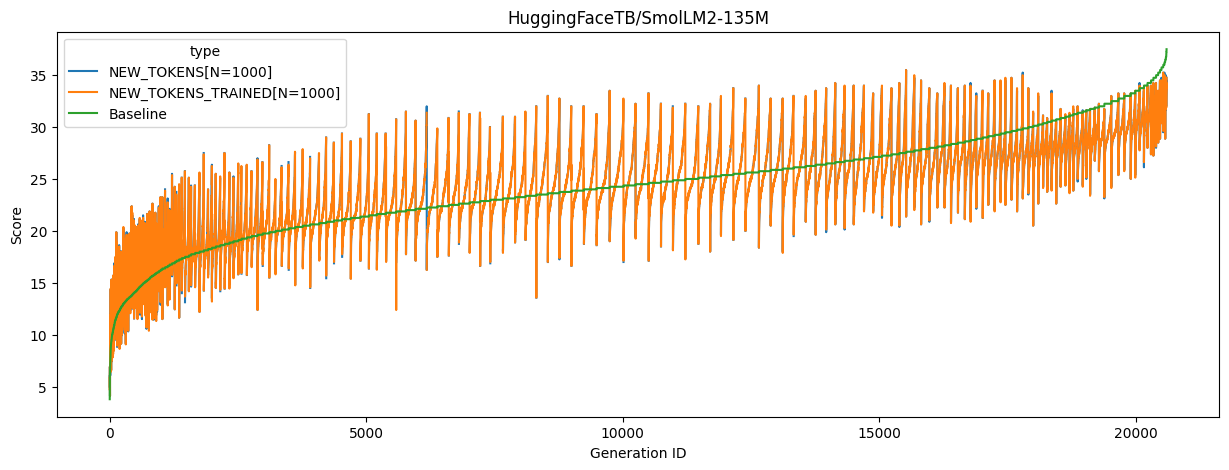
\includegraphics[width=\textwidth]{Figures/Appendix/token-rank-comparison_1000_smol135M.png}
    \caption[Score comparison for \textit{SmolLM2-135M} w/ 1000 new tokens]{Score comparison between original sub-token sequences and newly introduced tokens. Higher ranks indicate higher model preference.}
    \label{annex:fig:new_token_rank:1000_smol135M}
\end{figure}
\FloatBarrier
% ---------------------------------------------
\subsubsection{Number New Tokens = 5000}
\begin{figure}[H]
    \centering
    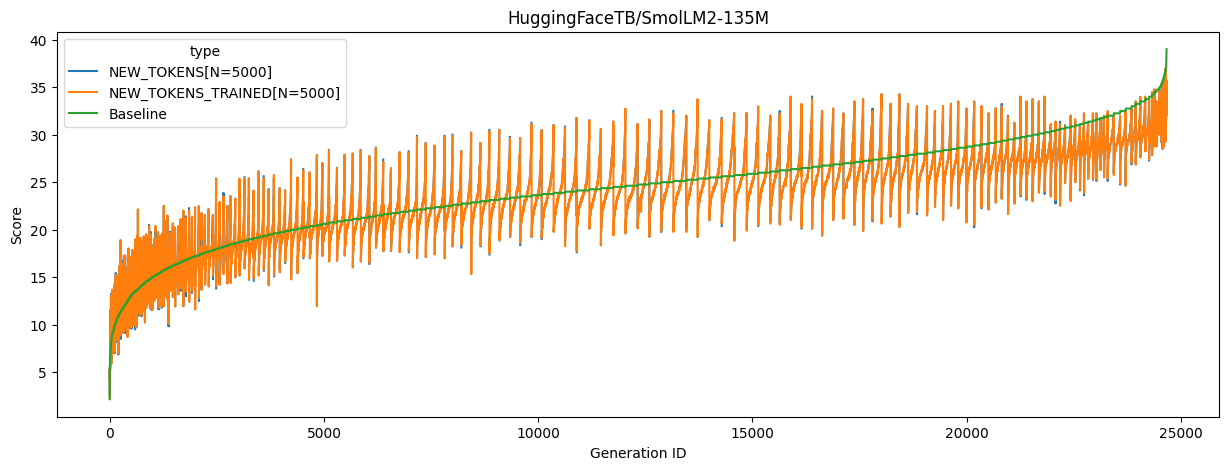
\includegraphics[width=\textwidth]{Figures/Appendix/token-rank-comparison_5000_smol135M.png}
    \caption[Score comparison for \textit{SmolLM2-135M} w/ 5000 new tokens]{Score comparison between original sub-token sequences and newly introduced tokens. Higher ranks indicate higher model preference.}
    \label{annex:fig:new_token_rank:5000_smol135M}
\end{figure}
\FloatBarrier
% ---------------------------------------------
\subsubsection{Number New Tokens = 7500}
\begin{figure}[H]
    \centering
    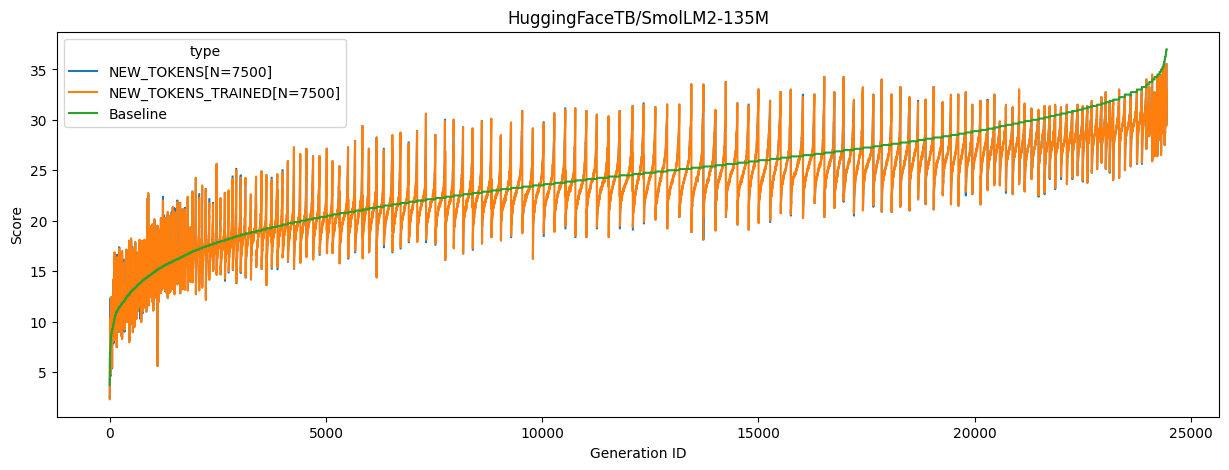
\includegraphics[width=\textwidth]{Figures/Appendix/token-rank-comparison_7500_smol135M.png}
    \caption[Score comparison for \textit{SmolLM2-135M} w/ 7500 new tokens]{Score comparison between original sub-token sequences and newly introduced tokens. Higher ranks indicate higher model preference.}
    \label{annex:fig:new_token_rank:7500_smol135M}
\end{figure}
\FloatBarrier
% ---------------------------------------------


% ======================================================================
\subsection{Model \textit{Qwen/Qwen2.5-1.5B-Instruct}}

% ---------------------------------------------
\subsubsection{Number New Tokens = 1000}
\begin{figure}[H]
    \centering
    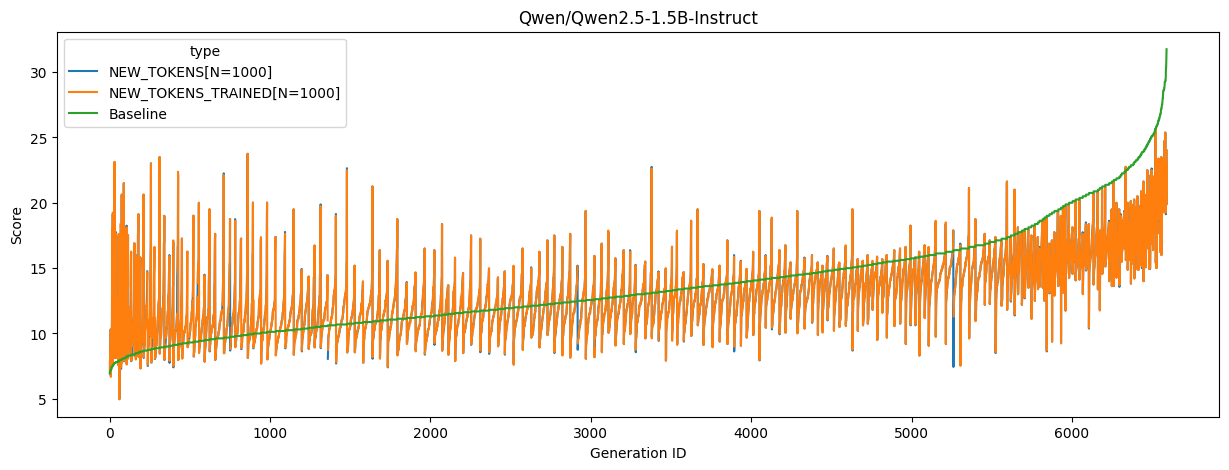
\includegraphics[width=\textwidth]{Figures/Appendix/token-rank-comparison_1000_qwen.png}
    \caption[Score comparison for \textit{Qwen2.5-1.5B-Instruct} w/ 1000 new tokens]{Score comparison between original sub-token sequences and newly introduced tokens. Higher ranks indicate higher model preference.}1`
    \label{annex:fig:new_token_rank:1000_qwen}
\end{figure}
\FloatBarrier
% ---------------------------------------------
\subsubsection{Number New Tokens = 5000}
\begin{figure}[H]
    \centering
    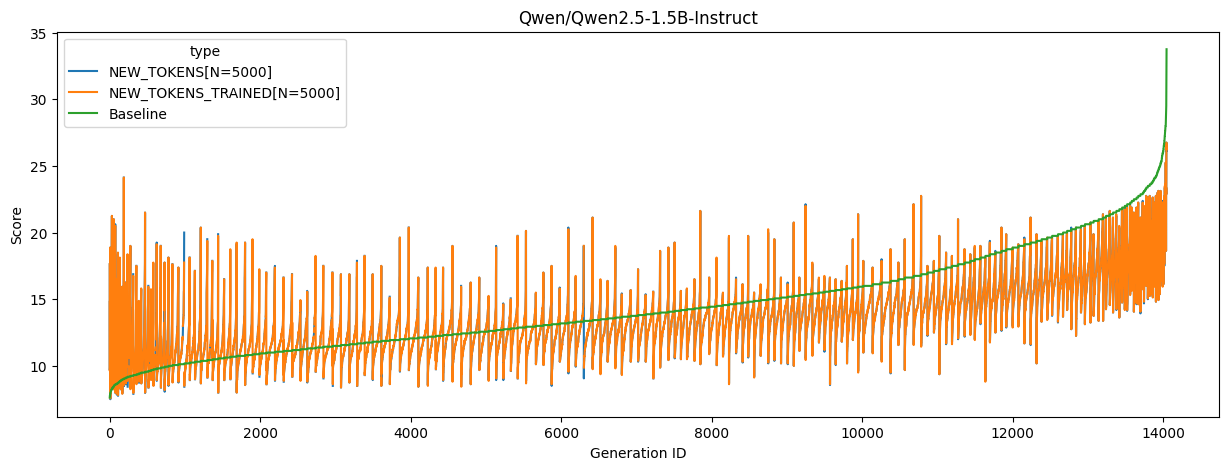
\includegraphics[width=\textwidth]{Figures/Appendix/token-rank-comparison_5000_qwen.png}
    \caption[Score comparison for \textit{Qwen2.5-1.5B-Instruct} w/ 5000 new tokens]{Score comparison between original sub-token sequences and newly introduced tokens. Higher ranks indicate higher model preference.}
    \label{annex:fig:new_token_rank:5000_qwen}
\end{figure}
\FloatBarrier
% ---------------------------------------------

\subsubsection{Number New Tokens = 7500}
\begin{figure}[H]
    \centering
    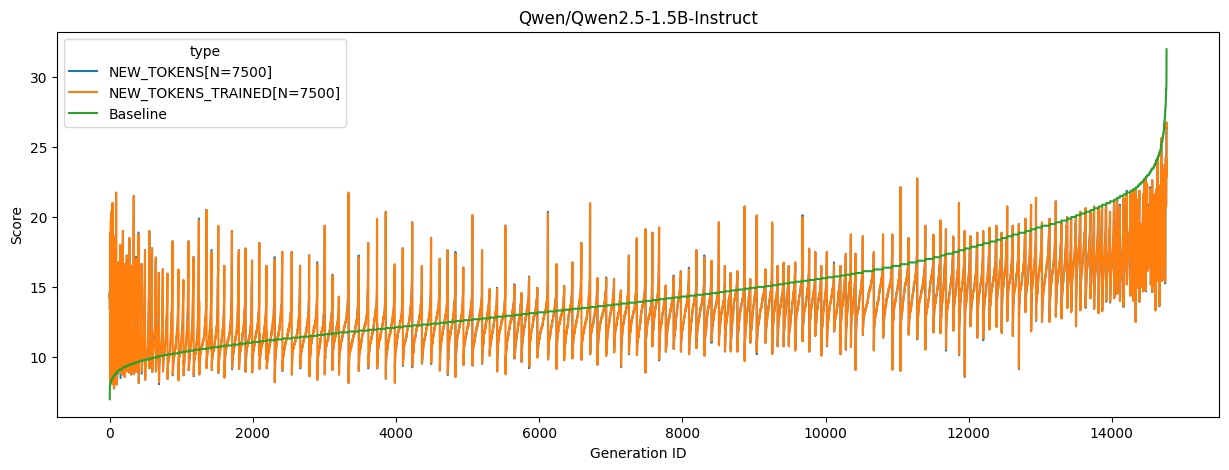
\includegraphics[width=\textwidth]{Figures/Appendix/token-rank-comparison_7500_qwen.png}
    \caption[Score comparison for \textit{Qwen2.5-1.5B-Instruct} w/ 7500 new tokens]{Score comparison between original sub-token sequences and newly introduced tokens. Higher ranks indicate higher model preference.}
    \label{annex:fig:new_token_rank:7500_qwen}
\end{figure}
\FloatBarrier
% ---------------------------------------------


% ======================================================================
\subsection{Model \textit{HuggingFaceTB/SmolLM3-3B}}

% ---------------------------------------------
\subsubsection{Number New Tokens = 1000}
\begin{figure}[H]
    \centering
    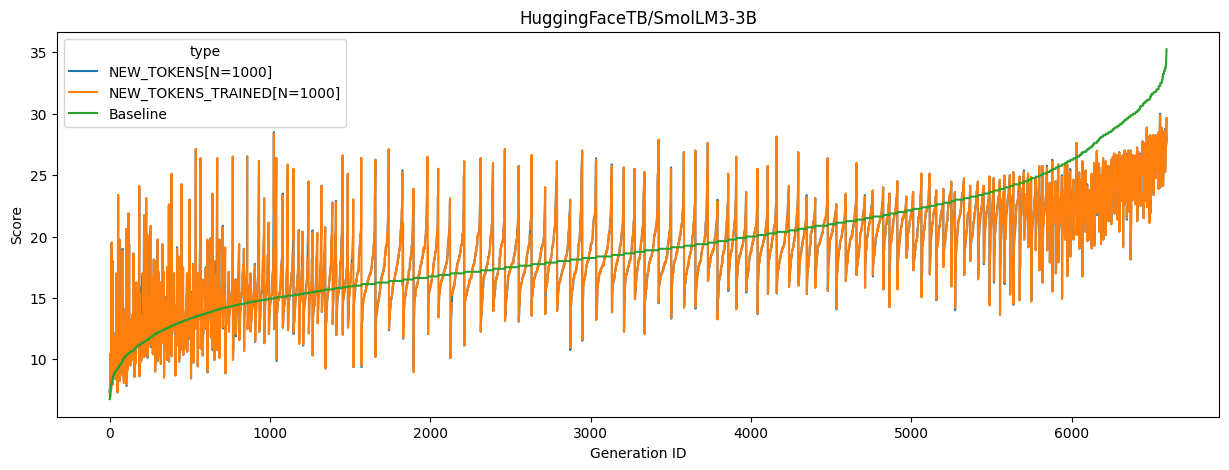
\includegraphics[width=\textwidth]{Figures/Appendix/token-rank-comparison_1000_smol3B.png}
    \caption[Score comparison for \textit{SmolLM3-3B} w/ 1000 new tokens]{Score comparison between original sub-token sequences and newly introduced tokens. Higher ranks indicate higher model preference.}
    \label{annex:fig:new_token_rank:1000_smol3B}
\end{figure}
\FloatBarrier
% ---------------------------------------------

\subsubsection{Number New Tokens = 5000}
\begin{figure}[H]
    \centering
    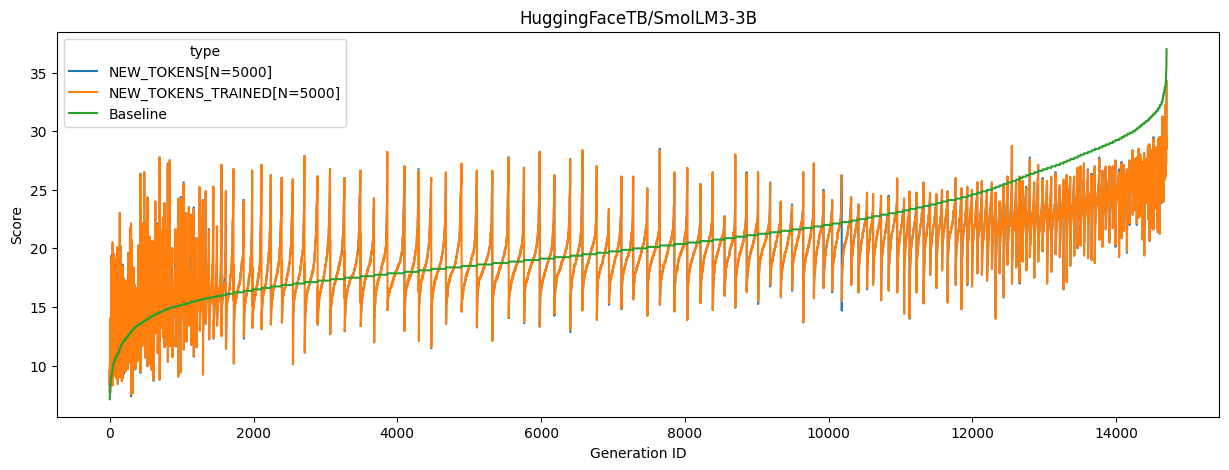
\includegraphics[width=\textwidth]{Figures/Appendix/token-rank-comparison_5000_smol3B.png}
    \caption[Score comparison for \textit{SmolLM3-3B} w/ 5000 new tokens]{Score comparison between original sub-token sequences and newly introduced tokens. Higher ranks indicate higher model preference.}
    \label{annex:fig:new_token_rank:5000_smol3B}
\end{figure}
\FloatBarrier
% ---------------------------------------------

\subsubsection{Number New Tokens = 7500}
\begin{figure}[H]
    \centering
    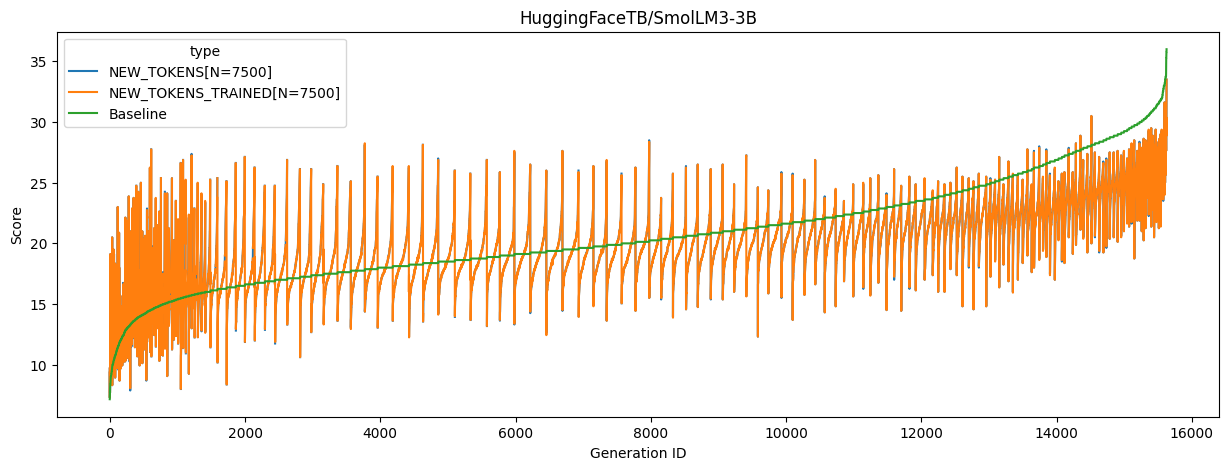
\includegraphics[width=\textwidth]{Figures/Appendix/token-rank-comparison_7500_smol3B.png}
    \caption[Score comparison for \textit{SmolLM3-3B} w/ 7500 new tokens]{Score comparison between original sub-token sequences and newly introduced tokens. Higher ranks indicate higher model preference.}
    \label{annex:fig:new_token_rank:7500_smol3B}
\end{figure}
\FloatBarrier
% ---------------------------------------------





% ======================================================================
% ======================================================================
% 
%
%                     Rank Diff Violin Distribution
%
%
% ======================================================================
% ======================================================================
\section{Rank Differences Distribution}
\label{annex:results-rank-differences}

Referenced on [\ref{subsec:rank-distributions}]


% ---------------------------------------------
\subsection{Model \textit{HuggingFaceTB/SmolLM2-135M}}
\begin{figure}[H]
    \centering
    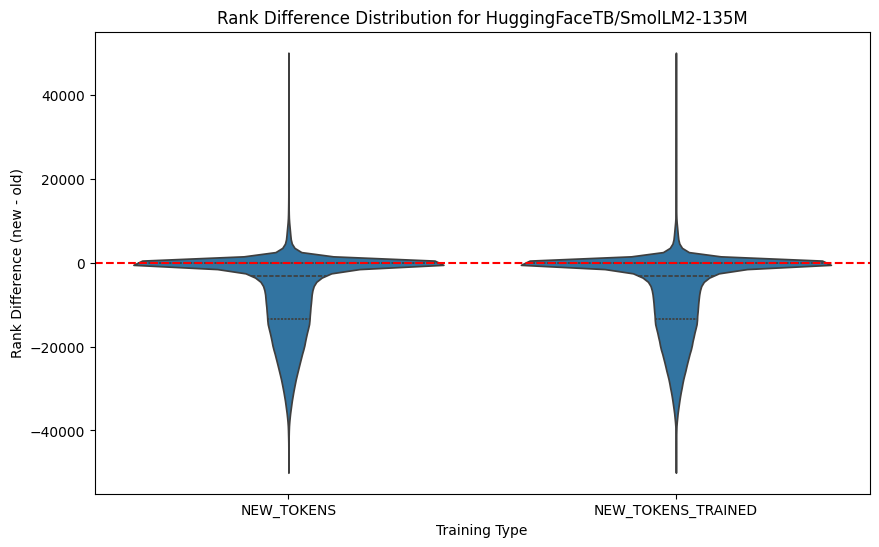
\includegraphics[width=1\textwidth]{Figures//Appendix/violin_smol135M.png}
    \caption[\text{ }\text{ }Distribution of Rank Differences for model \textit{SmolLM2-135M}]{Distribution of rank differences across the entire results data. Negative numbers show preference towards \texttt{new\_token}.}
    \label{annex:fig:violin_rank_dist:smol135M}
\end{figure}
% ---------------------------------------------


% ---------------------------------------------
\subsection{Model \textit{Qwen/Qwen2.5-1.5B-Instruct}}
\begin{figure}[H]
    \centering
    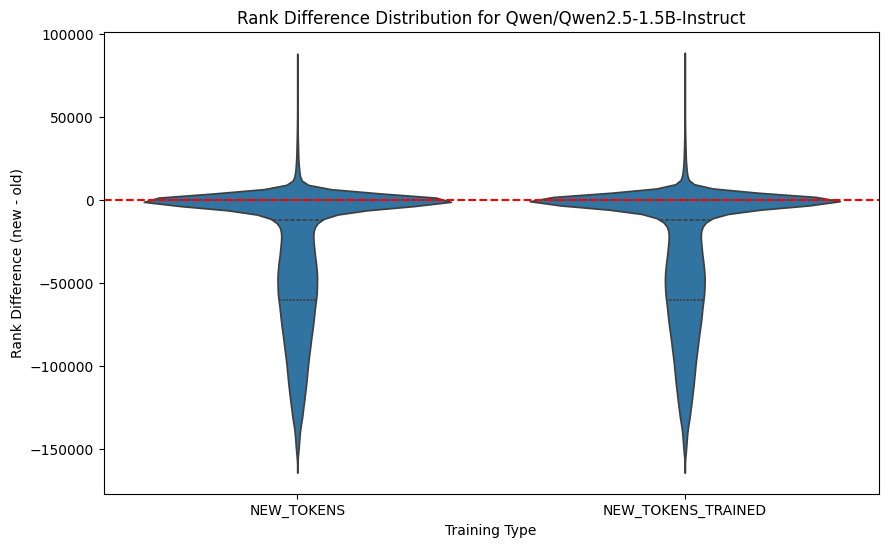
\includegraphics[width=1\textwidth]{Figures//Appendix/violin_qwen.png}
    \caption[\text{ }\text{ }Distribution of Rank Differences for model \textit{Qwen2.5-1.5B-Instruct}]{Distribution of rank differences across the entire results data. Negative numbers show preference towards \texttt{new\_token}.}
    \label{annex:fig:violin_rank_dist:qwen1.5B}
\end{figure}
% ---------------------------------------------


% ---------------------------------------------
\subsection{Model \textit{HuggingFaceTB/SmolLM3-3B}}
\begin{figure}[H]
    \centering
    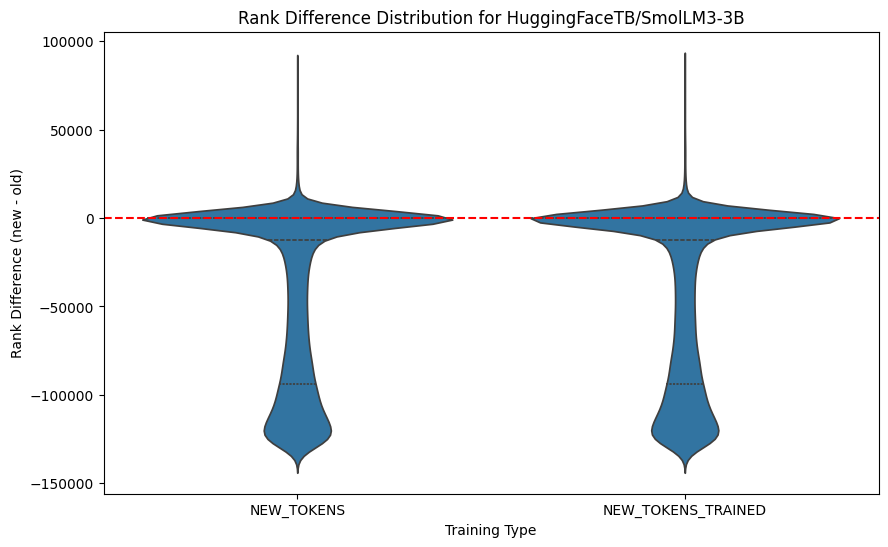
\includegraphics[width=1\textwidth]{Figures//Appendix/violin_smol3B.png}
    \caption[\text{ }\text{ }Distribution of Rank Differences for model \textit{SmolLM3-3B}]{Distribution of rank differences across the entire results data. Negative numbers show preference towards \texttt{new\_token}.}
    \label{annex:fig:violin_rank_dist:smol3B}
\end{figure}
% ---------------------------------------------